Die vorliegende Bachelorarbeit wird in Kooperation mit der Hochschule für Technik Stuttgart bei der NeuroCheck GmbH angefertigt.

\p
Die NeuroCheck GmbH ist ein Unternehmen, welches System- und Softwarelösungen im Fachgebiet der industriellen Bildverarbeitung anbietet.
Dabei blickt das Unternehmen mit Hauptsitz in Remseck am Neckar auf eine Firmengeschichte von über 25 Jahren zurück.
Mit nun mehr als 20000 verkauften Applikationen in über 40 Ländern sowie mehreren Partnerunternehmen im Ausland haben die NeuroCheck-Systeme weltweit Anwendungen gefunden.

\p
Mithilfe der NeuroCheck-Software ist es möglich, automatisierte Sichtprüfungen zur Qualitätskontrolle durchzuführen.
Hierfür lassen sich vom Anwender komplexe Prüfprogramme nach einem Baukastenprinzip erstellen.
Dadurch entstehen vielseitige An\-wen\-dungs\-mög\-lich\-kei\-ten.
Diese schaffen weite Teile der Industriebranchen als mögliche Kunden, unter anderem die Automobilindustrie, die Elektronikbranchen und die Medizintechnik.

% Abbildung: NeuroCheck Logo
\begin{figure}[H]
	\centering
	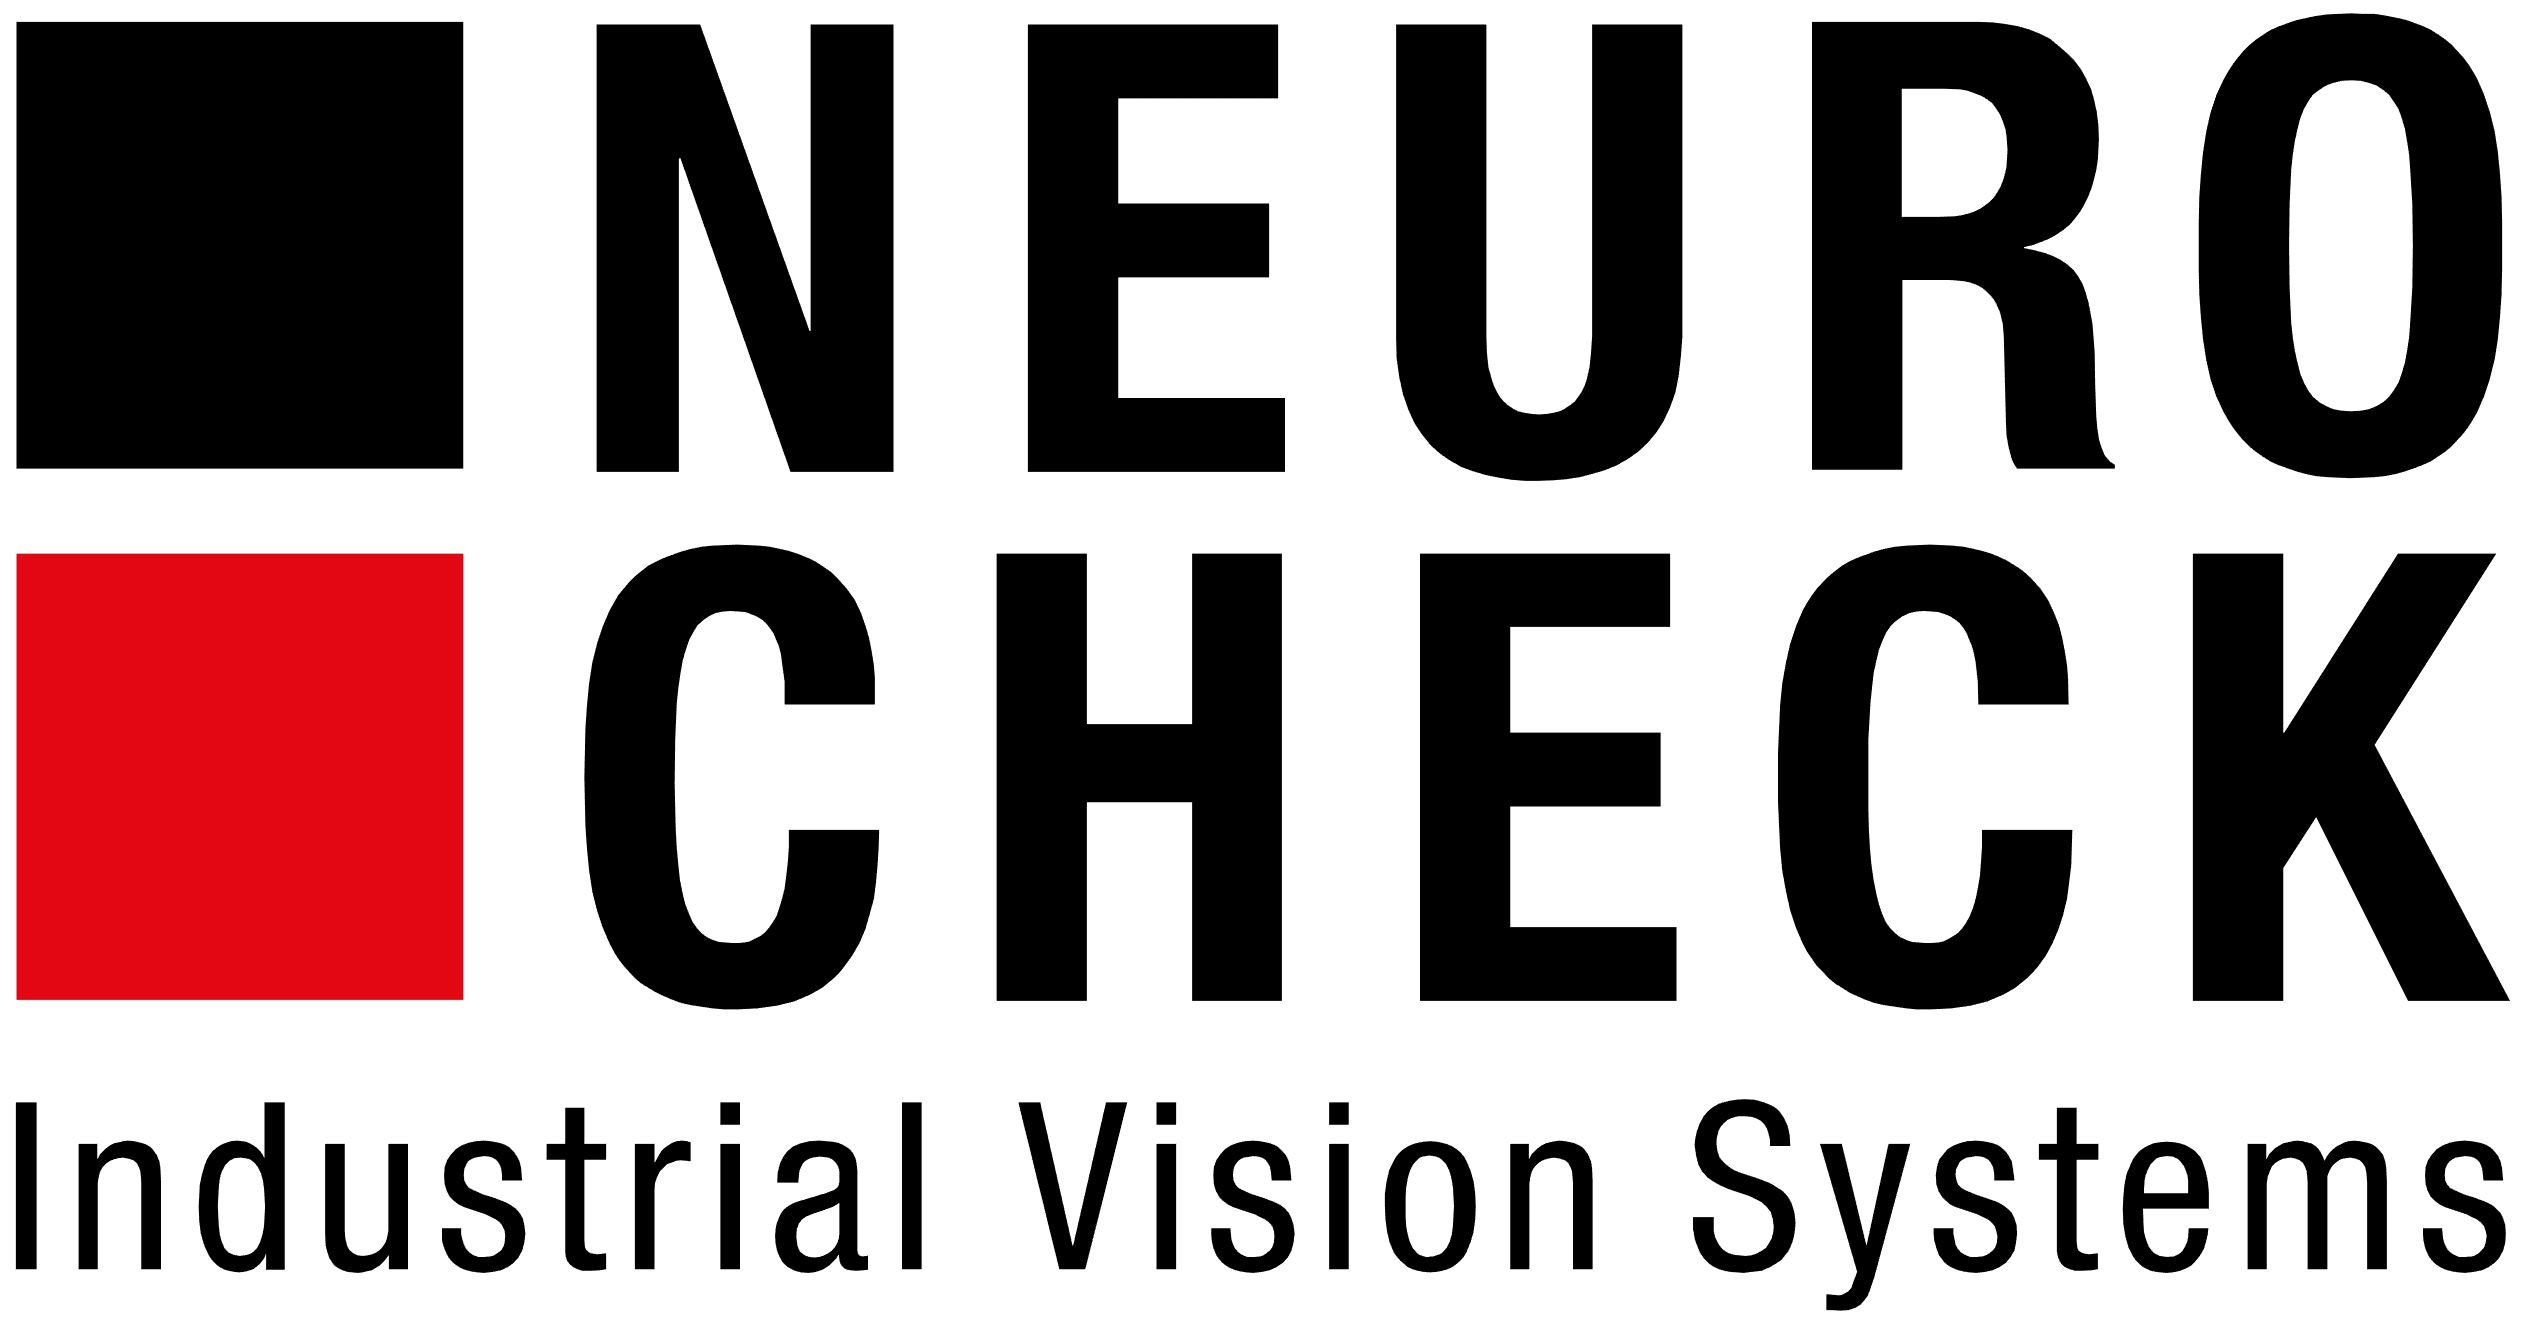
\includegraphics[width=0.3\textwidth]{01_einfuehrung/unternehmensvorstellung/figures/neurocheck_logo}
	\caption[NeuroCheck Logo]{NeuroCheck Logo \cite{nclogo}}
\end{figure}